\documentclass[sigconf]{acmart}
\renewcommand\footnotetextcopyrightpermission[1]{}
\settopmatter{printacmref=false}
\setcopyright{none}
\pagestyle{plain}

\usepackage{hyperref}
\usepackage[hyphenbreaks]{breakurl}
\usepackage{balance}
\usepackage{url}
\usepackage{color}
\usepackage{caption}
\usepackage{diagbox}
\usepackage{subfigure}
\usepackage{multirow}
\usepackage{booktabs}
\usepackage{epsfig,endnotes}
\usepackage{enumitem}
\usepackage{multirow}
\usepackage{booktabs}
\newcommand{\RNum}[1]{\uppercase\expandafter{\romannumeral #1\relax}}

\newcommand{\model}{{\mathcal{F}_{\theta}}}
\newcommand{\orgmodel}{{\mathcal{F}_{o}}}
\DeclareMathOperator{\sign}{sign}


\DeclareMathOperator*{\argmin}{argmin}

\newcommand{\para}[1]{{\vspace{2pt} \noindent \textbf{#1}
    \hspace{6pt}}}

\newcommand{\subpara}[1]{{\vspace{1.0pt} \textbf{#1}
    \hspace{4pt}}}

\newcommand{\fixme}[1]{{\color{red} #1}}
\newcommand{\rewrite}[1]{{\color{black} #1}}
\newcommand{\todo}[1]{{\color{red}TODO:  #1}}
\newcommand{\wip}[1]{{\color{gray} #1}}

\newcommand{\askben}[1]{{\color{red} Q:  #1}}
\newcommand{\emily}[1]{{\color{black} #1}}

\newcommand{\arjun}[1]{{\color{black} Arjun:  #1}}

\definecolor{applegreen}{rgb}{0.55, 0.71, 0.0}

\newcommand{\abedit}[1]{{\color{black} #1}}
\newcommand{\shawnmr}[1]{{\color{black} #1}}
\newcommand{\shawn}[1]{{\color{black} #1}}
\newcommand{\rev}[1]{{\color{black} #1}}


\newcommand{\htedit}[1]{{\color{black} #1}}

\newcommand{\bencheck}[1]{{\color{black} #1}}

\newcommand{\ssedit}[1]{{\color{black} #1}}
\newcommand{\outline}[1]{{\color{blue} #1}}
\newcommand{\ol}[1]{{\color{blue} #1}}

\newcommand{\etal}{{\em et al.\ }}
\newcommand{\eg}{{\em e.g.,\ }}
\newcommand{\ie}{{\em i.e.,\ }}

\newcommand{\secspace}{\vspace{-0.05in}}
\newcommand{\secspacesm}{\vspace{0.0in}}

\newcommand{\system}{{\em Neo}}

\newcommand{\ad}[1]{{$\mathcal{A}$}}
\newcommand{\service}[1]{{$\mathcal{S}$}}
\newcommand{\mcD}{\mathcal{D}}

\newcommand{\ytface}{{\tt YTFace}}
\newcommand{\cifarS}{{\tt CIFAR10}}
\newcommand{\cifar}{{\tt CIFAR10}}
\newcommand{\skin}{{\tt SkinCancer}}

\newcommand{\cifarL}{{\tt CIFAR100}}

\newcommand{\imagenet}{{\tt ImageNet}}

\newenvironment{packed_itemize}{
\begin{list}{\labelitemi}{\leftmargin=0.5em}
  \setlength{\itemsep}{1pt}
  \setlength{\parskip}{0pt}
  \setlength{\parsep}{0pt}
  \setlength{\headsep}{0pt}
  \setlength{\topskip}{0pt}
  \setlength{\topmargin}{0pt}
  \setlength{\topsep}{0pt}
  \setlength{\partopsep}{0pt}
}{\end{list}}

\newenvironment{packed_enumerate}{
\begin{enumerate}
 \setlength{\itemsep}{1pt}
 \setlength{\parskip}{0pt}
 \setlength{\parsep}{0pt}
 \setlength{\headsep}{0pt}
 \setlength{\topskip}{0pt}
 \setlength{\topmargin}{0pt}
 \setlength{\topsep}{0pt}
 \setlength{\partopsep}{0pt}
}{\end{enumerate}}

\begin{document}
\title{A Response to Glaze Purification via IMPRESS}

\author{Shawn Shan$^\dag$, Stanley Wu$^\dag$, Haitao Zheng, Ben Y. Zhao\\
$^\dag$ denotes authors with equal contribution\\
  {\em Department of Computer Science, University of Chicago}\\
  {\em \{shawnshan, stanleywu, htzheng, ravenben\}@cs.uchicago.edu}}

\begin{abstract}

  Recent work proposed a new mechanism to remove protective perturbation
  added by Glaze in order to again enable mimicry of art styles from images
  protected by Glaze.  Despite promising results shown in the original paper,
  our own tests with the authors' code demonstrated several limitations of
  the proposed purification approach.  The main limitations are 1)
  purification has a limited effect when tested on artists that are \textit{not
    well-known historical artists} already embedded in original training
  data, 2) problems in evaluation metrics, and 3) 
  collateral damage on mimicry result for clean images.  We believe these
  limitations should be carefully considered in order to understand real
  world usability of the purification attack.

\end{abstract}

\maketitle

\section{Introduction}
\label{sec:intro}


Transformers, in particular decoder-only models (e.g.\ GPT~\citep{brown2020language}, Llama~\citep{touvron2023llama}) which process input sequences in a causal fashion, are one of the main drivers of modern deep learning's success.
Numerous approaches attempt to approximate the core attention layer to address its efficiency issues~\citep{tay2022efficient}, such as scaling quadratically in sequence length during training and requiring a cache of size linear in sequence length during autoregressive generation.
In parallel, a class of alternative sequence models, structured state-space models (SSMs), have emerged with linear scaling in sequence length during training and constant state size during generation.
They show strong performance on long-range tasks (e.g. S4~\citep{gu2022efficiently}) and recently matched or beat Transformers on language modeling (e.g. Mamba \citep{gu2023mamba}) at small to moderate scale.
However, the development of SSMs have appeared disjoint from the community's collective effort to improve Transformers, such as understanding them theoretically as well as optimizing them on modern hardware.
As a result, it is more difficult to understand and experiment with SSMs compared to Transformers, and it remains challenging to train SSMs as efficiently as Transformers from both an algorithmic and systems perspective.


Our main goal is to develop a rich body of theoretical connections between structured SSMs and variants of attention.
This will allow us to transfer algorithmic and systems optimizations originally developed for Transformers to SSMs, towards the goal of building foundation models that perform better than Transformers while scaling more efficiently in sequence length.
A milestone contribution in this direction was the \textbf{Linear Attention (LA)} framework \citep{katharopoulos2020transformers},
which derived a connection between autoregressive attention and linear RNNs
by showing the equivalence between ``dual forms'' of quadratic kernelized attention and a particular linear recurrence.
This duality allows new capabilities such as the ability to have both efficient parallelizable training and efficient autoregressive inference.
In the same spirit, this paper provides multiple viewpoints connecting linear-complexity SSMs with quadratic-complexity forms to combine the strengths of SSMs and attention.%
\footnote{Technically speaking, these connections only relate to certain flavors of attention; the title of this paper is an homage to \citet{katharopoulos2020transformers} which first showed that ``Transformers are RNNs''.}

\iftoggle{arxiv}{
\begin{wrapfigure}{R}{0.48\linewidth}
  \begin{center}
    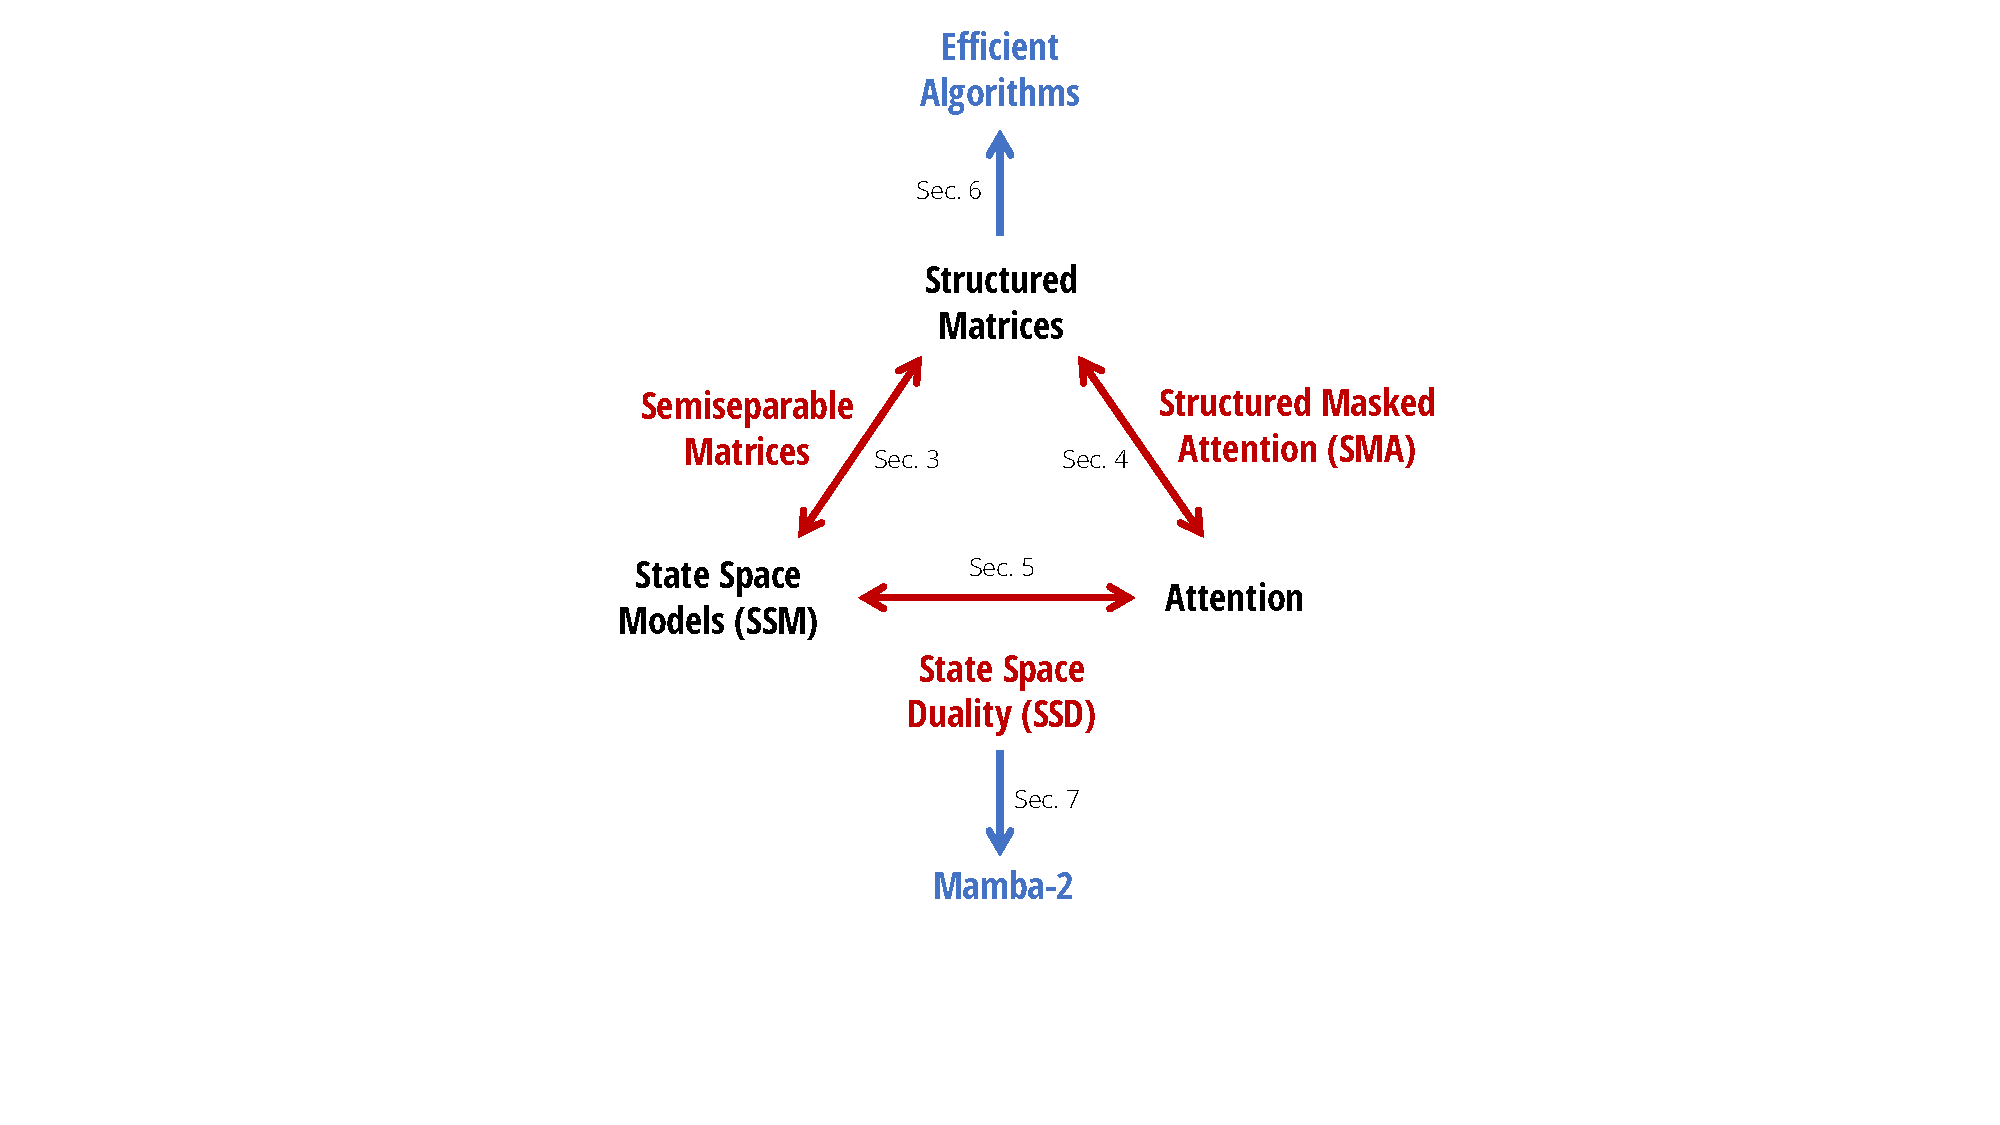
\includegraphics[width=\linewidth]{fig/ssd_roadmap.pdf}
  \end{center}
  \caption{
    (\textbf{Structured State-Space Duality}.)
    This paper fleshes out the relationship between state space models and attention through the bridge of structured matrices.
  }
  \label{fig:roadmap}
\end{wrapfigure}
}{}

\para{State Space Duality.}
Our framework connecting structured SSMs and variants of attention, which we call \textbf{structured state space duality} (SSD),
is made through the abstractions of \textbf{structured matrices}:
matrices with subquadratic parameters and multiplication complexity.
We develop two broad frameworks for representing sequence models, one as matrix transformations and one as tensor contractions, which each reveal different perspectives of the duality.
Our technical contributions include:
\begin{itemize}[leftmargin=*,itemsep=0pt,topsep=0pt]
  \item We show an equivalence between state space models and a well-studied family of structured matrices called \textbf{semiseparable matrices}\iftoggle{arxiv}{ (\cref{sec:ssm})}{}.
    This connection is at the heart our framework, revealing new properties and algorithms for SSMs. A central message of this paper is that \emph{different methods of computing state space models can be reframed as various matrix multiplication algorithms on structured matrices}.
  \item We significantly improve the theory of linear attention~\citep{katharopoulos2020transformers}.
    We first provide an incisive proof of its recurrent form through the language of tensor contractions, and then generalize it to a new family of \textbf{structured masked attention (SMA)}\iftoggle{arxiv}{ (\cref{sec:attention})}{}.
  \item We connect SSMs and SMA, showing that they have a large intersection that are duals of each other, possessing both SSM-like linear and attention-like quadratic forms\iftoggle{arxiv}{ (\cref{sec:ssd})}{}.
    \iftoggle{arxiv}{We also prove that any kernel attention method possessing a fast recurrent form must be an SSM.}{}
\end{itemize}


Beyond its intrinsic theoretical value, our framework opens up a broad set of directions for understanding and improving sequence models.

\para{Efficient Algorithms.}
First and most importantly, our framework exposes new efficient and easily-implementable algorithms for computing SSMs\iftoggle{arxiv}{ (\cref{sec:efficient})}{}.
We introduce a new \textbf{SSD algorithm}, based on block decompositions of semiseparable matrices, that takes advantage of both the linear SSM recurrence and quadratic dual form, obtaining optimal tradeoffs on all main efficiency axes (e.g. training and inference compute, memory usage, and ability to leverage matrix multiplication units on modern hardware).
A dedicated implementation of SSD is $2-8\times$ faster than the optimized selective scan implementation of Mamba, while simultaneously allowing for much larger recurrent state sizes ($8\times$ the size of Mamba or even higher, with minimal slowdown).
SSD is highly competitive with optimized implementations of softmax attention (FlashAttention-2~\citep{dao2023flashattention2}), crossing over at sequence length 2K and 6$\times$ faster at sequence length 16K.


\iftoggle{arxiv}{
\para{Architecture Design.}
One major obstacle to adopting new architectures such as SSMs is the ecosystem tailored to Transformers, such as hardware-efficient optimization and parallelism techniques for large-scale training.
Our framework allows using established conventions and techniques for attention to build a vocabulary of architecture design choices for SSMs, and further improve them (\cref{sec:architecture}).
For example, we introduce the analog of heads from multi-head attention (MHA) to SSMs.
We show that the Mamba architecture is a \textbf{multi-input SSM (MIS)} that turns out to be analogous to \textbf{multi-value attention (MVA)}, and compare other variants of Mamba with different head structures.

We also use these ideas to make slight modifications to the Mamba block, which allows tensor parallelism to be implemented (e.g. in the style of Megatron~\citep{shoeybi2019megatron}).
The main ideas include introducing grouped-value attention (GVA) head structure, and moving all data-dependent projections to occur in parallel at the beginning of the block.


}{
  \para{Mamba-2.}
  Additionally, inspired by the connection between SSMs and Transformers, we slightly modify the neural network architecture of Mamba by moving all data-dependent projections to occur in parallel at the beginning of the block. %
}
The combination of the modified parallel Mamba block, together with using SSD as the inner SSM layer, results in the \textbf{Mamba-2} architecture.
We investigate Chinchilla scaling laws for Mamba-2 in the same setting as Mamba, finding that it Pareto dominates Mamba and Transformer++ in both perplexity and wall-clock time.
We additionally train a family of Mamba-2 models at varying sizes on the Pile, showing that it matches or outperforms Mamba and open source Transformers on standard downstream evaluations.
For example, Mamba-2 with 2.7B parameters trained on 300B tokens on the Pile outperforms Mamba-2.8B, Pythia-2.8B and even Pythia-6.9B trained on the same dataset.

\iftoggle{arxiv}{
\paragraph{Systems Optimizations.}
The SSD framework connects SSMs and Transformers, allowing us to leverage a rich body of work on systems optimizations developed for Transformers~(\cref{sec:systems}).
\begin{itemize}[leftmargin=*,itemsep=0pt,topsep=0pt]
  \item For example, Tensor Parallelism (TP) is an important model parallelism technique to train large Transformer models by splitting each layer across GPUs on the same node.
    We design Mamba-2 to be TP-friendly, reducing the number of synchronization point per block by half.
  \item For very long sequences whose activations do not fit on one device, sequence parallelism has been developed for the attention blocks.
    We describe how to train SSMs in general and Mamba-2 in particular with sequence parallelism, by passing the recurrent states between devices.
  \item For finetuning with examples of different lengths, for best efficiency, Transformer requires sophisticated techniques to remove padding tokens and perform attention on variable length sequences.
    We show how Mamba-2 can be trained with variable sequence lengths efficiently, requiring no padding tokens.
\end{itemize}
}{}

\cref{sec:experiments} empirically validates Mamba-2 on language modeling, training efficiency, and a difficult multi-query associative recall task~\citep{arora2024simple}.
Finally, in \cref{sec:related}, we provide an extended related work and discuss potential research directions opened up by our framework.

Model code and pre-trained checkpoints are open-sourced at \url{https://github.com/state-spaces/mamba}.







\section{Background and Related Work}
\label{sec:back}

We begin by providing background on style mimicry and existing image-based protection methods. Then we follow with an overview of publicly available tools that enable style mimicry attacks on the video domain.

\subsection{Style Mimicry and Existing Defenses}
\label{sec:back1}
In a style mimicry attack, a bad actor finetunes a text-to-image model to
generate art in a particular artist's style without their consent. 
Since the introduction of text-to-image diffusion~\cite{sd-release,podell2023sdxl,df,novelai-update,ramesh2022hierarchical} models in 2022, style mimicry has grown significantly. There have been multiple high-profile mimicry incidents involving human artists~\cite{hollie-steal,sarah-andersen,lensa-steal,sam-steal}, and new companies are founded that focus purely on style mimicry~\cite{aigame,lexica}. AI marketplaces have also recently gained traction, with websites like CivitAI~\cite{civitai} offering over 119K ready-to-use mimicry models for people to download and use.

\para{Image-based style mimicry. } 
Style mimicry relies on finetuning pretrained text-to-image models (\eg stable diffusion) on a small set of images from a specific style~\cite{ruiz2022dreambooth,finetune-c,gal2022image}. The quality of these images greatly impacts the mimicry result, and thus, attackers often scrape high quality images from artists' websites and online galleries~\cite{hollie-steal,sam-steal}. In practice, a bad actor does not need many (less than 20 images~\cite{shan2023glaze,gal2022image}) in order to successfully generate arbitrary artwork from a victim artist's style. Because of the risk of image-based mimicry, many artists choose to reduce the amount of art they post online~\cite{aiprotest}, reduce the quality of any posted art~\cite{lowres}, and apply protection (discussed in details below) on this artwork~\cite{shan2023glaze}. 

\para{Protecting images from style mimicry. } 
Existing work (Mist~\cite{mist}, Anti-Dreambooth~\cite{antidb}, and Glaze \cite{shan2023glaze}) has 
proposed methods that leverage clean-label poisoning~\cite{saha2020hidden, turner2018clean, zhu2019transferable} to prevent style mimicry. At a high level, these systems add small optimized perturbations to image artwork that modifies the perturbed image's feature space representation without altering its content. The altered feature space representation prevents models from learning the correct artistic style. In general, these protection tools calculate the perturbation $\delta_x$ for an image $x$ using the following objective: 

\secspace
\begin{eqnarray}
   &\min\limits_{\delta_x} Dist\left( \Phi(x + \delta_x), \Phi(T)\right),  \label{eq:cloakopt}\\
  & \text{subject to } \; |\delta_x|< p, \nonumber
\end{eqnarray} 

where $\Phi$ is a generic image feature extractor from a public text-to-image model, $Dist(.)$ computes the distance between two feature representations, $|\delta_x|$ measures the perceptual perturbation caused by protection, and $p$ is the perceptual perturbation budget. $T$ is 
a ``target image'' that the perturbation $\delta_x$ is optimized towards, such that $x + 
\delta_x$ resembles $T$ in feature space while being visually identical to $x$. Mist~\cite{mist} extends the optimization objective across the entire diffusion process, including gradient computations through the randomized diffusion denoising process. By default, Mist uses a predefined black and white patterned image as its target with the goal of producing chaotic patterns in generated images. Anti-DB (Anti-Dreambooth)~\cite{antidb} is most similar to Mist, but modifies the optimization objective to specifically target Dreambooth~\cite{ruiz2022dreambooth} text-to-image models. There, they find that training surrogate models alongside computing image perturbations results in stronger protection, though it incurs additional computation time. Glaze~\cite{shan2023glaze} introduces input-specific target images by performing style transfer on the input image using a contrasting artistic style. This method preserves the overall content of the input image, while changing mainly the style, which the authors argue leads to more robust protection. Glaze then attacks the image encoder of a diffusion model as detailed above. 

These protection tools have been positively received by the artist community,
with Glaze having been downloaded at least 2.3 million
times~\cite{shan2023glazewebsite}. While these systems are typically too
computationally expensive for artists, efforts have been made to improve
accessibility~\cite{mistgithub, shan2023webglaze}. Since these systems are
free and increasingly available, images may no longer be a viable data source
for attackers to access artwork for fine-tuning text-to-image models. 

Video protection, on the other hand, has yet to be explored. Computation time per image is already limiting for many artists, and applying the same algorithms to all frames would be many times more costly. Yet, videos represent a significant source of data, incentivizing attackers to explore publicly available video art, such as short animation, movies or video game trailers etc..

Until recently, most style mimicry models are trained on still images. This 
is no longer the case today because 1) artists are increasingly more reluctant to post their 
work on the Internet~\cite{aiprotest}, 2) existing defenses (\S\ref{sec:back1}) are effective at protecting still images against mimicry, 3) video frames offer a significantly more diverse range of images compared to still images. 

\para{Video content is a promising source for mimicry. } 
Video content (\eg game trailers, anime, short videos, documentary, ads) provides promising alternative data sources for two reasons. First, video contents often offer a more diverse (3D) shots of an object or style, \eg rotating shot of an object, panning across a scene. These diverse viewpoints 
enable models to better learn the content during the training process~\cite{videomotivate}. Second, there are significantly more video frames compared to still images and many of the videos contain unique art styles/characters. The entire Internet produces around 3.2 billions still images daily~\cite{manyvideos}, while YouTube alone sees over 271,000 hours of videos (\ie around 29 billions video frames) uploaded per day. Specifically, gaming companies and animation studios often use short videos as a way to promote new games, characters, and movies. Movie clip compilations and trailers are readily available on YouTube~\cite{movietrailers}, while video game companies like Riot and Mihoyo frequently post teasers and trailers showcasing new playable content, or highly anticipated characters~\cite{genshintrailer, leaguetrailer}. These videos are filled with original artwork, and contain image frames that are prime targets for style mimicry. 

\para{Video-based mimicry in the real-world. } 
Style mimicry using video content has already occurred in the real-world. Bad actors have created and distributed software that generates high quality text-to-image datasets from online videos. One GitHub tool~\cite{anime2sd} automates the process of downloading (\eg torrenting) Japanese Anime episodes and extracting high quality frames of desired characters. Another option~\cite{civitai-video} advertised on CivitAI does the same, with the additional capability of scraping frames from screencap websites such as FanCaps~\cite{fancaps}. These tools demonstrate that there already exists sophisticated technology aimed at creating text-to-image datasets from original video content. 

We also provide our own examples of this threat. We download and extract high quality frames from YouTube videos and train style mimicry models on them (Figure~\ref{fig:style-mimicry-scenario}). Figure~\ref{fig:style-mimicry-baseline} shows some examples of extracted video frames as well as mimicry results generated by the style mimicry model. We include human evaluation of the success of these style mimicry images later using user studies with both artists and the general public in \S\ref{sec:eval}. 

While there has been recent developments in text-to-video~\cite{videoworldsimulators2024} and image-to-video models~\cite{blattmann2023stable}, we leave them as a topic for future work, and focus solely on text-to-image mimicry where the source of data originates from video content. 


\secspace
\section{Evaluation of IMPRESS}
\label{sec:issues}

Here, we first identify a few flaws in IMPRESS's experiment setup 
and then evaluate purification performance 
in several realistic mimicry scenarios. 

\para{Setup. } We follow the purification setup from the original IMPRESS paper and the source
code provided by the authors. We use default 
Glaze setup (perturbation budget = $0.07$) as described in the paper. 
We follow style mimicry setup in prior 
work~\cite{shan2023glaze}. Given a set of artworks, we mimic its style by
fine-tuning stable diffusion model (version 1.5) using DreamBooth 
for 600 to 1000 steps depending on the finetuning sample size for the artist.

\begin{figure*}
  \centering
  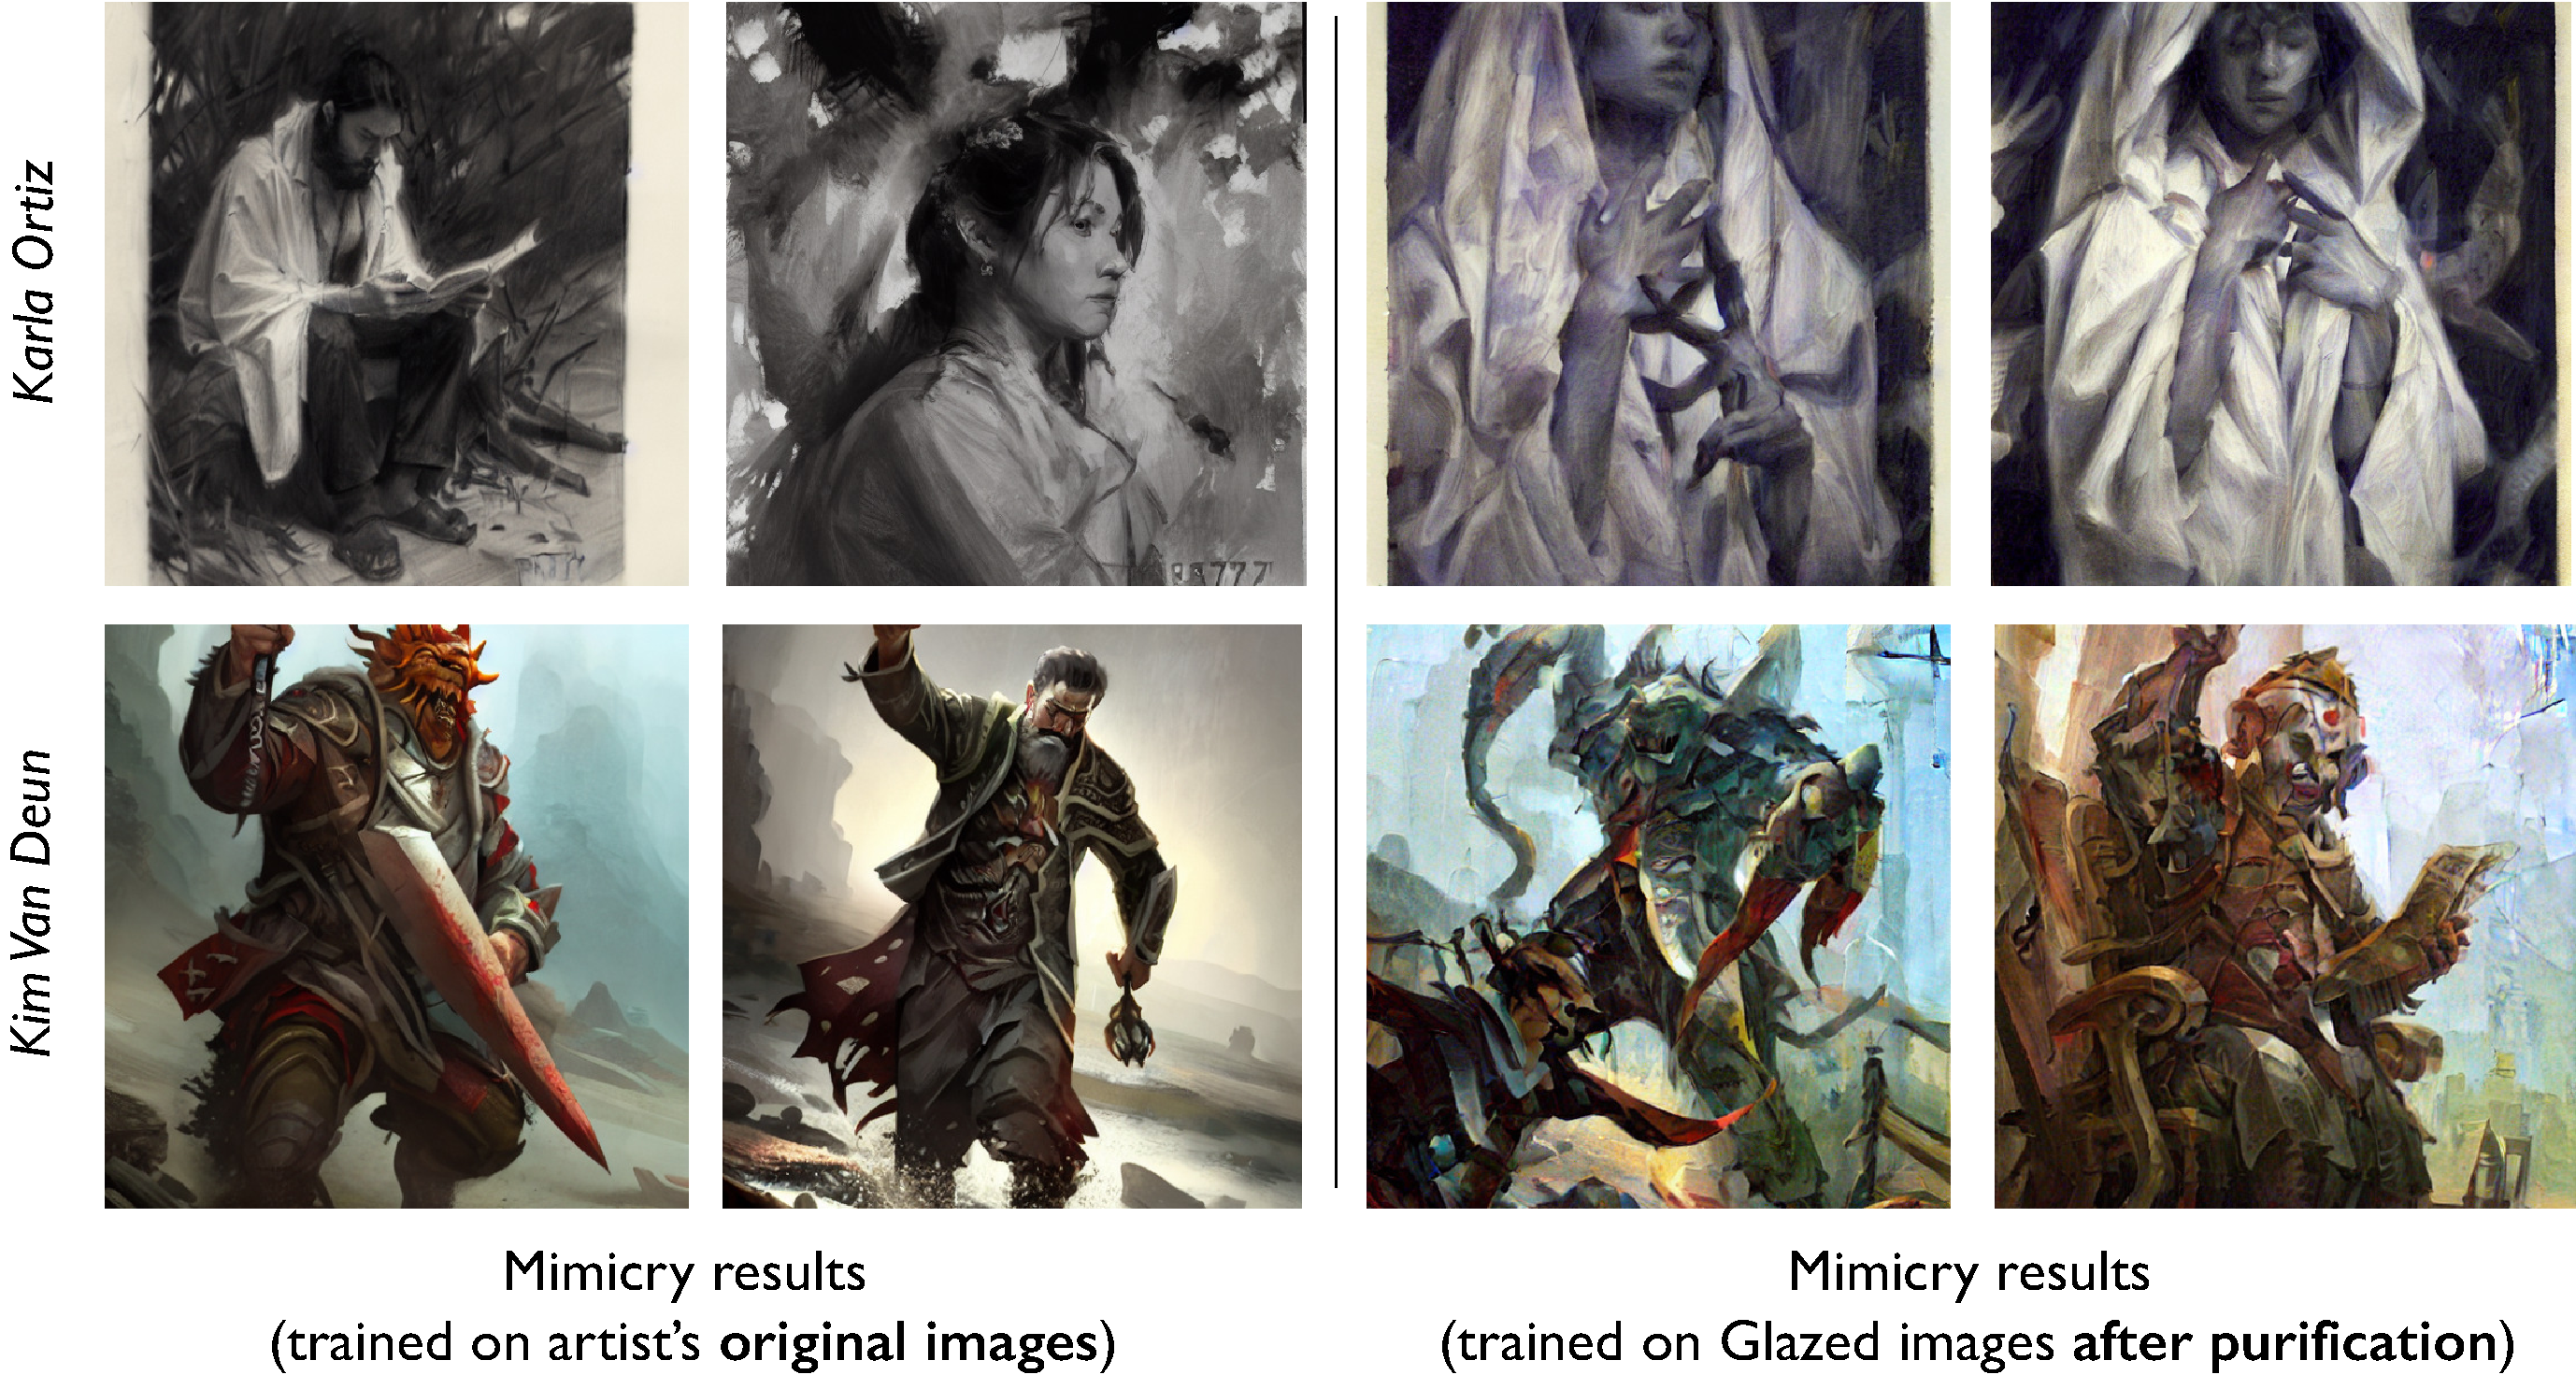
\includegraphics[width=0.99\linewidth]{nonhistorical.pdf}
  \vspace{-0.1in}
  \caption{Mimicry results on non-historical artists (Karla Ortiz and Kim van Deun). Left shows the images generated from a model trained on original images; right shows the images generated from a model trained on images that are first Glazed and then purified by IMPRESS. }
  \label{fig:non-historical}
  \vspace{-0.in}
\end{figure*}

\begin{figure*}
  \centering
  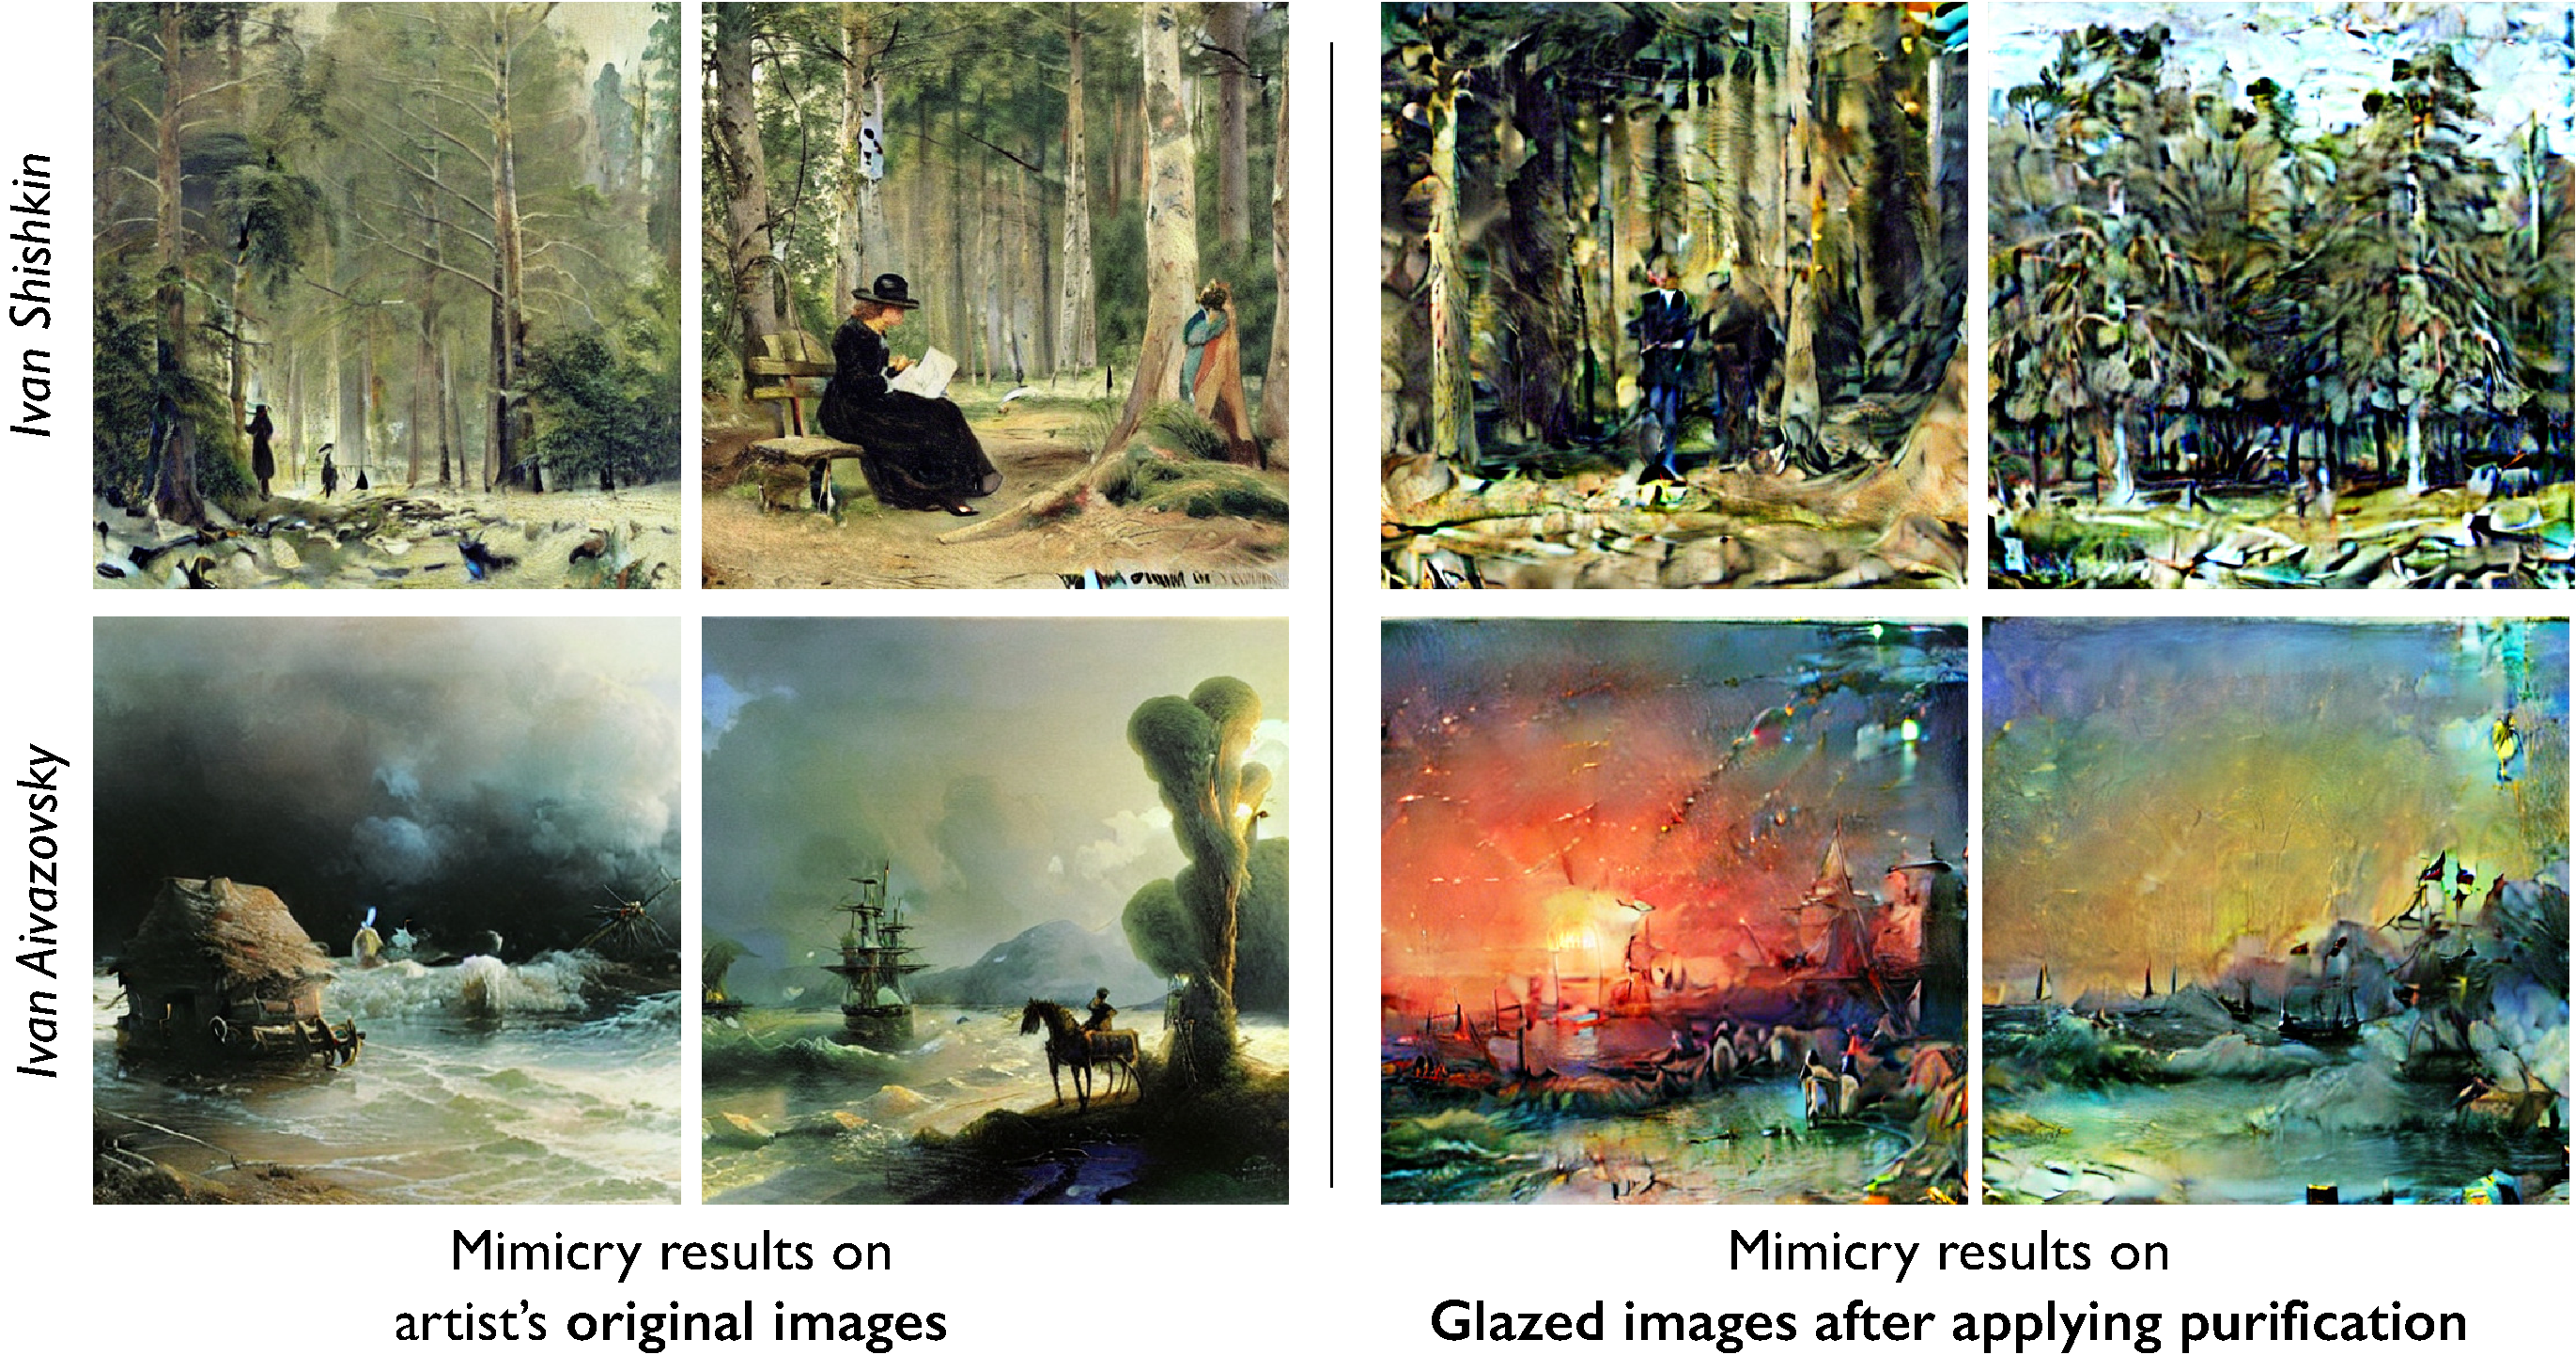
\includegraphics[width=0.99\linewidth]{smooth.pdf}
  \vspace{-0.1in}
  \caption{Mimicry results on smooth surface art styles (Ivan Shishkin and Ivan Aivazovsky). Left shows the images generated from a model trained on original images; right shows the images generated from a model trained on images that are first Glazed and then purified by IMPRESS. }
   \label{fig:smooth}
  \vspace{-0.in}
\end{figure*}

\begin{figure*}
  \centering
  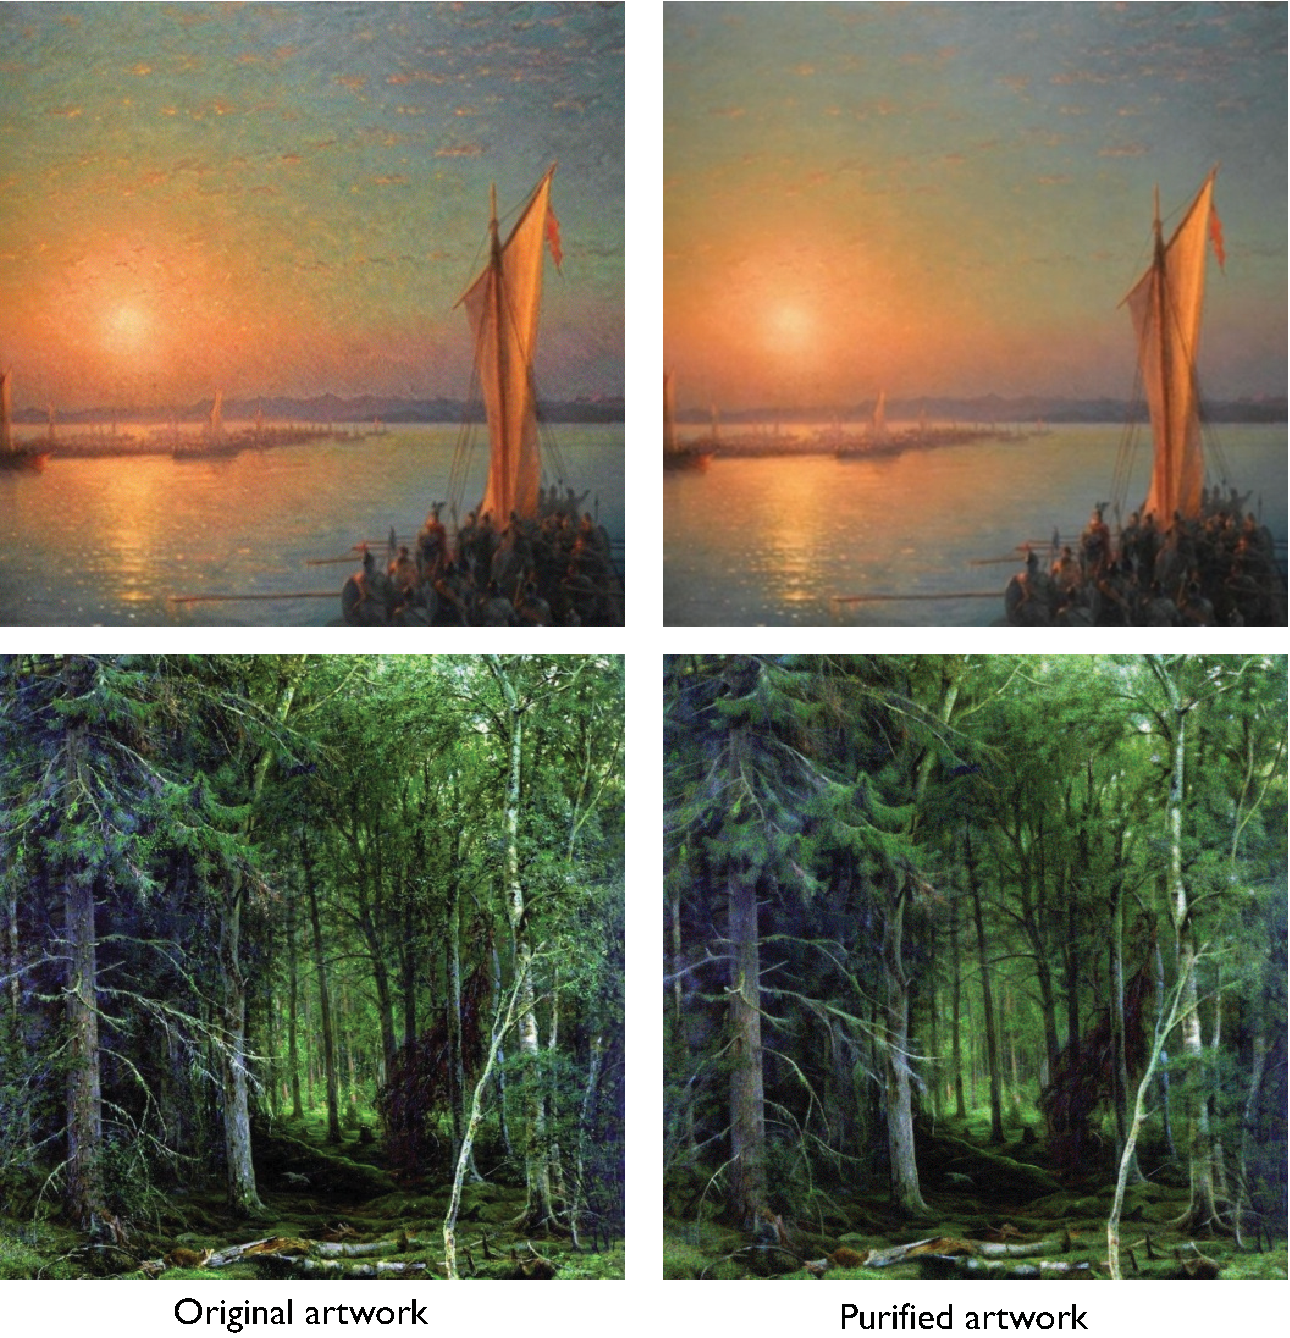
\includegraphics[width=0.95\linewidth]{clean-degrade.pdf}
  \vspace{-0.1in}
  \caption{Original artwork and corresponding purified artwork. }
  \label{fig:clean}
  \vspace{-0.in}
\end{figure*}

\subsection{Generalizability to Realistic Scenarios}

In the original IMPRESS paper, the authors focus the evaluation on protecting the
art styles of famous historical artists (Monet, Van Gogh) -- whose style are already learned
by pretrained diffusion models prior to style mimicry. In the real-world, it is current artists
who are most concerned about AI mimicking their art style. Glaze is designed
to protect those artists, and they are not as heavily pretrained into the
base model as Monet or Van Gogh. 

We evaluate IMPRESS on non-historical artists and show that purification
has limited effectiveness at removing Glaze protection. 
Even for historical artists, we find the purification works poorly for 
certain art styles. Lastly, we find purification also degrades clean image quality where
it removes texture from art pieces. 

\para{Performance on non-historical artists. } We use artwork from Karla 
Ortiz and Kim Van Deun to simulate the mimicry attack on current artists. Karla is a fine-art artist 
with a similar style as some historical artists tested in the IMPRESS paper. 
Figure~\ref{fig:non-historical}
shows the mimicry results when model trained on artist's original art pieces (left)
or when model trained on art pieces that are first Glazed
and then purified by IMPRESS (right). We can observe significant amount of 
artifacts on mimicry results when the model is trained on purified Glazed images. 

\para{Poor performance on certain art styles. } IMPRESS works by adding artifacts
on Glazed images to recover the latent representation of original artwork. 
We found purification has more challenges recovering smooth surface 
art styles (realism art, symbolism, romanticism, etc) even for historical
artists already trained into the base model. 
We choose two historical artists: Ivan Aivazovsky (romanticism style) and Ivan Shishkin (realism style). 

Figure~\ref{fig:smooth} shows the mimicry results. We see IMPRESS 
introduces signficiant amount of artifacts to the mimicked images. 
The weaker performance is likely because purifying  the 
original smoother surface art requires the optimization to 
be very percise -- find the exact smooth surface. 

\para{Degrading image quality. } We found the purification process degrades 
clean image quality. Figure~\ref{fig:clean} shows original artwork 
and its corresponding purified artwork. The purified artwork is much more
blurry as purification removes textures from the images. 

\subsection{CLIP-based metrics are Inaccurate}

``CLIP genre accuracy'' quantifies if mimicked art is classified into the same art genre as the original 
art pieces according to a CLIP model. It has been used in prior work to evaluate mimicry 
success. However, in our own tests dating back to late September 2023, we
found CLIP genre accuracy is a poor indicator of end-to-end mimicry success.  
CLIP accuracy is especially poor when evaluating attacks against Glaze. The 
reason is that attacks (such as 
IMPRESS purification), as they seek to remove Glaze effect from art, often have signficant impact 
on the base image quaility of the artwork. 
The degradation in image quality is not captured by CLIP accuracy, \eg a very
low quality cubism painting is still classified as ``cubism'' with high
probability. But the result are not successful 
mimicry due to the low quaility of the mimicked images. 
Because of these poor properties as an accuracy indicator, we stopped using
CLIP distance as a success metric starting with the Glaze v1.1 update
(October 2023). 

\section{Discussion}
\label{sec:discussion}

We discuss related work, limitations, and some future directions.

\paragraph{Related Work.}
\cref{sec:discussion:selection} discusses how the selection mechanism relates to similar concepts.
\cref{sec:related} has an extended related work of SSMs and other related models.

\paragraph{No Free Lunch: Continuous-Discrete Spectrum.}
Structured SSMs were originally defined as discretizations of continuous systems \eqref{eq:ssm},
and have had a strong inductive bias toward continuous-time data modalities such as perceptual signals (e.g.\ audio, video).
As discussed in \cref{sec:method:motivation,sec:method:properties}, the selection mechanism overcomes their weaknesses
on discrete modalities such as text and DNA;
but this conversely can impede their performance on data that LTI SSMs excel on.
Our ablations on audio waveforms examine this tradeoff in more detail.

\paragraph{Downstream Affordances.}
Transformer-based foundation models (particularly LLMs) have a rich ecosystem of properties and modes of interaction with pretrained models,
such as fine-tuning, adaptation, prompting, in-context learning, instruction tuning, RLHF, quantization, and so on.
We are particularly interested in whether Transformer alternatives such as SSMs have similar properties and affordances.

%

\paragraph{Scaling.}
Our empirical evaluation is limited to small model sizes,
below the threshold of most strong open source LLMs (e.g. Llama \citep{touvron2023llama})
as well as other recurrent models such as RWKV~\citep{peng2023rwkv} and RetNet~\citep{sun2023retentive},
which have been evaluated at the 7B parameter scale and beyond.
It remains to assess whether Mamba still compares favorably at these larger sizes.
We also note that scaling SSMs may involve further engineering challenges and adjustments to the model
that are not discussed in this paper.

%


\bibliographystyle{ACM-Reference-Format}
\bibliography{impress}
\balance

\end{document}

\typeout{get arXiv to do 4 passes: Label(s) may have changed. Rerun}
